
\chapter{Architectures of Graph Neural Networks}

\section*{Abstract}

As deep learning algorithms increasingly adress graph-structured data, Graph Neural Networks (GNNs) play a more and more important role in various fields, including computational chemistry and the prediction of molecular properties. However, currently in the literature different architectures and approaches of GNNs exist. Therefore, this paper analyzes the current state-of-art by exploring architectures and approaches of GNNs in the literature. By creating an overview, it will show that convolutional GNNs are commonly used and particulary reliable when working with molecular properties. With the help of structured process CRISP-DM, later a convolutional GNN will be developed that predicts the potential energy surface of molecules with the QM9 dataset and a simpler water dataset. The evaluation shows high accuracy, therefore the GNN was succesfully developed. \\

\textit{\textbf{Keywords:} graph neural networks, architectures, literature review, potential energy surface prediction}

\section{Introduction}
While deep learning algorithms effectively capture hidden patterns of Euclidean data, there is an increasing number of application areas where the data is represented in the form of graphs or structures similar to graphs \cite{wu_comprehensive_2021}. Due to the expressive capabilities of graphs, researches on analyzing these kind of structures with machine learning have been receiving more and more attention. This is evident in the areas of social science, such as social networks, natural science like physical systems, knowledge graphs and other research areas \cite{zhou_graph_2020}. Deep learning based methods that operate in a graph domains are called Graph Neural Networks (GNNs) \cite{velickovic_everything_2023}. \\ 
In computational chemistry, molecules are modeled as graphs enabling various experiments \cite{wu_comprehensive_2021}. This includes the prediction of potential energy surfaces for  molecules made of hydrogen compounds or other materials \cite{liu_computational_2023}. In the current literature, different approaches or architectures for GNNs exist \cite{wu_comprehensive_2021}. This raises the question of which approaches are available and which of these approaches is well suited for the prediction of molecular properties such as potential energy surfaces. \\

In order to solve the presented problem, the following research question and sub-questions are created: 
\begin{center}
    \textit{"How can a Graph Neural Network for the prediction of molecular properties be developed?"} \\
\end{center}
Q1: \textit{What approaches for Graph Neural Networks currently exist in the Literature?} \\
Q2: \textit{What architecture suits the prediction of molecular properties best?} \\

The goal of this paper is to develop an understanding of graph neural networks in general and the different types of architectures that exist in the literature. Besides, in the scope of this thesis, an understanding of the prediction of potential energy is created. Based on this procedure, the literature review will show what architecture of graph neural networks suits the prediction of potential energy best. In summary, to answer the developed research question and sub-questions, the following artifacts will be created as part of the research: 

\begin{itemize}
    \item literature review of different graph neural network architectures
    \item prototypical implementation of a graph neural network for the potential energy prediction
\end{itemize}  

The structure of this paper is as followed: first, the scientific foundations and theoretical background are discussed. Then the research methodology is presented in detail. Based on this, the findings and their results are presented and then discussed. Finally, a conclusion and discussion of the results is provided, as well as an overview of possible research topics based on this work.  

\section{Theoretical Background}
\subsection{Graph Neural Networks}

Graph Neural Networks (GNNs) are a type of neural networks that are used to work with graph-structured data. They provide a framework for tasks that focus on learning dependencies and interactions between data points. GNNs use the structure of graphs to capture and process information in way that is not possible using traditional neural networks \cite{duvenaud2015convolutional}. In the context of GNNs a graph consists of nodes that represent entities and edges that describe relationships between those entities. The objective of GNNs is to learn important node representations that contain both local and global graph information. \cite{wu_comprehensive_2021} GNNs are effective in dealing with non-Euclidean and irregular data structures. This makes GNNs very suitable for domains where relationships between data points are as important as, or even more important then, the individual data points itself \cite{zhou_graph_2020}. \\

The architecture of a GNN consists of layers that update node representations by aggregating information from neighboring nodes iteratively. This process enables nodes to relearn their understanding of the local context while considering the wider structure of the graph. The aggregation step involves weighted summation or concatenation of features from neighboring nodes, allowing each node to summarize information from its surroundings. \cite{velickovic_everything_2023, xu_how_2019} A key aspect of a GNN is the neighborhood aggregation function, which is also known as the message-passing mechanism \cite{gasteiger_directional_2022}. This function defines how information between nodes in each layer is exchanged. The power of GNNs lies in their ability to progressively enhance node representations through multiple layers, capturing detailed dependencies within the graph. 

\subsection{Potential Energy Surface Prediction}
The potential energy surface (PES), in the context of molecules and atoms, describes the energy of a molecule in regard to certain parameters, e.g. to the position of its atoms.    
Predicting the potential energy surface of atoms is a task in computational chemistry and materials science. It gives information about the stability and properties of molecules and materials \cite{liu_computational_2023}. This is helpful when to decide whether materials can be used to enable efficient catalytic processes in the field of hydrogen production \cite{chen_waste-derived_2023}. 

\section{Research Methodology}
First, the given problem of the prediction of molecular properties with GNNs was investigated. For this purpose, an initial investigation of the literature took place and the topic was explored. This is followed by the definitions of the research questions as well as the sub-questions and the delineation of the research topic. \\

\begin{figure}[h]
    \centering
    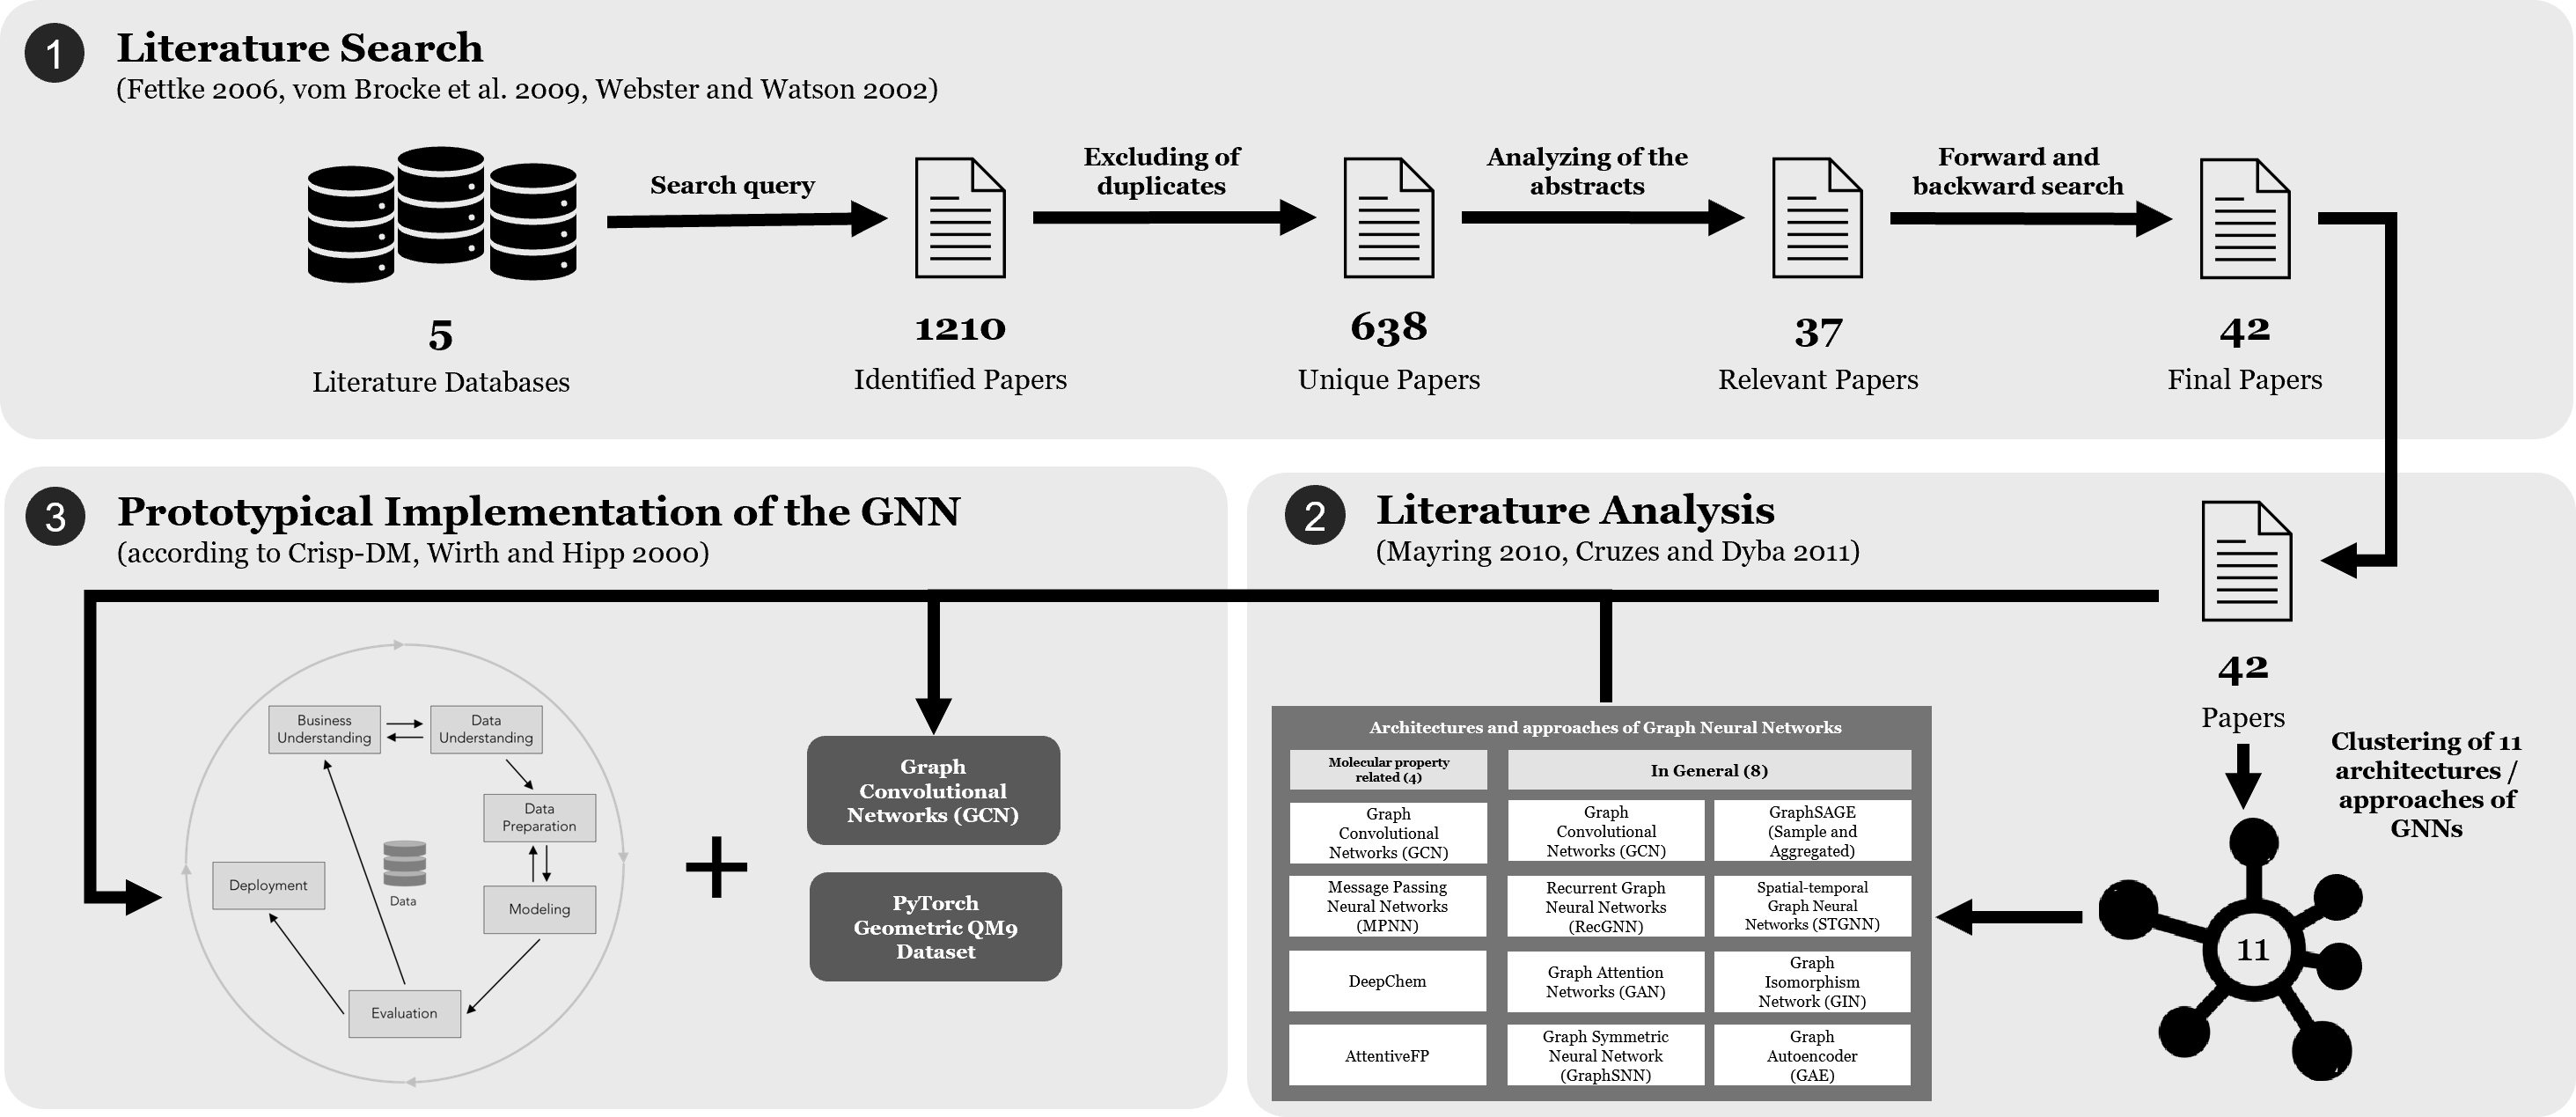
\includegraphics[width=0.95\textwidth]{02_paper01RM.png}
    \caption[Overview of the conducted research process]{\label{img:paper01rm}{Overview of the conducted research process}}
    \end{figure} 

Afterwards, a comprehensive and structured literature review is conducted with the aim of identifying different approaches of GNNs and finding the most suitable for molecular property prediction. The findings of this literature review are used for the creation of a common understanding of GNNs in the given context. In the next step, a GNN is prototypically implemented with the available dataset. This serves the goal of being able to directly test and evaluate the developed GNN. For better structuring and traceability of the procedure, the exact research process is shown in Figure \ref{img:paper01rm}, which is also described in detail in the following section. \\

In the \textbf{first step}, the literature search based on Fettke \cite{fettke_state---art_2006}, vom Brocke et al. \cite{vom_brocke_reconstructing_nodate} and Webster and Watson \cite{webster_analyzing_2002} was performed. The following literature databases were used: IEEE Xplore Digital Library, ScienceDirect, SpringerLink, Emeralt Insight and Google Scholar. Electronic searches of titles using the search terms [("Graph Neural Networks") AND (("architectures") OR ("approaches"))] and [("Graph Neural Networks") AND ("*molecular*")]. Moreover, no specific period of time was selected. According to the search query performed, these searches resulted in a total of 1210 publications. After analyzing abstract and keywords, 37 relevant publications remained for the given research focus. In addition to the database search, Webster and Watson \cite{webster_analyzing_2002} recommend performing a forward and backward search. These were performed in a final step and increased the number of final publications to 42. \\

In the \textbf{second step}, a total number of 42 papers were read in full and coded. For the clustering of the architectures and approaches of GNNs the procedure of Fettke \cite{fettke_state---art_2006} was performed. After this process of clustering, a total of 11 different architectures and approaches for GNNs could be identified. According to the research topic, this results are assigned into two different higher-level categories, "molecular property related" and "In General". \\

The \textbf{third step} covers the prototypical implementation of the GNN for molecular property prediction. Based on the findings of the literature review, a GNN is implemented and evaluated that predicts potential energy surfaces with the QM9 Dataset from Pytorch Geometric \cite{noauthor_torch_geometricdatasetsqm9_nodate}. The implementation of the GNN follows the established procedure of CRISP-DM \cite{wirth2000crisp} and is explained later in this paper. 

\section{Findings}
In this section, the results and findings are presented and discussed in detail. Especially the literature review and the prototypical implementation of the GNN for the prediction of potential energy will be considered. 


\subsection{Literature Review}

After the conduction of the literature review, two categories of GNN architectures and approaches could be identified, namely "molecular property related" and "In General". The first category lists all GNN architectures that are applied in computational chemistry, especially in working with molecular properties. The second category "In General"  describes general GNN architectures that occur in literature and also for other application areas. For both categories, different architectures and approaches were found, which are shown in Figure \ref{img:paper01findings}. In the following, the findings will be explained in more detail.

\begin{figure}[h]
    \centering
    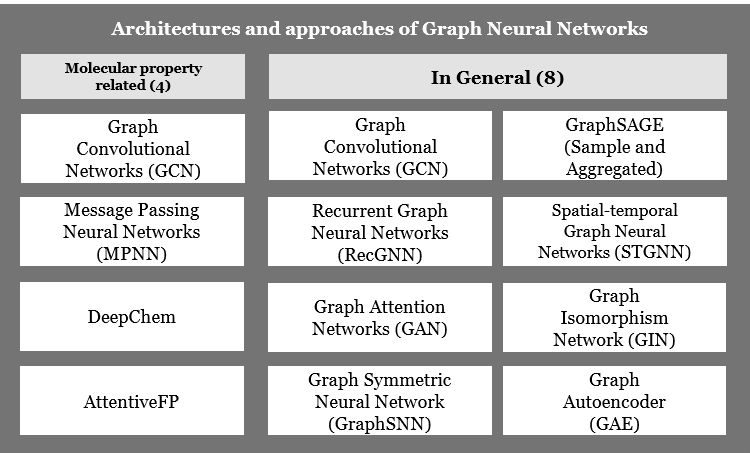
\includegraphics[width=0.95\textwidth]{03_lr_ergebnisse.png}
    \caption[Overview over die identified architectures and approaches for GNNs]{\label{img:paper01findings}{Overview over die identified architectures and approaches for GNNs}}
\end{figure} 

For the processing of data related to molecular property or computational chemistry, in the literature for different types of GNN approaches could be identified: Graph Convolutional Networks (GCN), Message Passing Neural Networks (MPNN), DeepChem and AttentiveFP. \\

Proposed by Gilmer et al. in 2020 \cite{gilmer_neural_2017}, Message Passing Neural Networks (MPNNs) are a class of graph neural networks designed for processing graph-structured data, targeting the application areas of chemistry and molecular property prediction. The architecture of MPNNs consists of message passing, updating node and edge representations iteratively through message passing functions, enabling the model to capture relationships reliable within the graph. The key components include message passing, aggregation, and readout. During message passing, information from neighboring nodes and edges is aggregated and transformed through learnable functions. Aggregation mechanisms, often involving summation or attention, allow nodes to incorporate information from their local environments. A readout function then processes the final node representations to make predictions about the entire graph. This design enables MPNNs to effectively handle variable-sized graphs and adapt to diverse molecular structures. \\

Unlike the other findings, DeepChem is no GNN itself, but a Python library for machine learning and deep learning on molecular and quantum datasets. The library consists of a extensive toolkit for working with molecular property prediction and related tasks \cite{noauthor_deepchem_nodate}. For example, DeepChem offers different deep learning models, including graph convolutional networks, graph attention networks, and recurrent neural networks. DeepChem is used for research in the field of computational chemistry and drug discovery \cite{altae-tran_low_2017}. \\

AttentiveFP is a deep learning model for graph data, which integrates attention mechanisms into GNNs.  In the area of computational chemistry, AttentiveFP captures and values the importance of specific atoms in a molecule. This model gives attention weights to highlight relevant atoms during information aggregation. In this way, the model is able to focus on specific regions within a molecular graph. The architecture of AttentiveFP involves message-passing steps where atoms exchange information based on their local environments. The attention mechanism assigns an importance scores to neighboring atoms, enabling the model to prioritize interactions between them. The focus on local context is particularly beneficial when handling various molecular structures. The attention-based approach enhances the capacity to recognize subtle chemical patterns, making it useful for applications in computational chemistry. According to its architecture, AttentiveFP is a specific Graph Attention Network (GAN). \cite{xiong_pushing_2019,jiang_could_2021} \\

The literature review showed that Convolutional Graph Neural Networks (GCNs) are both used for working in the field of molecular property prediction and in other application areas. Introduced by Kipf and Welling in 2016 \cite{kipf2016semi} GCNs are one of the earliest and commonly used architectures of GNNs \cite{wu_comprehensive_2021}. 

\begin{figure}[h]
    \centering
    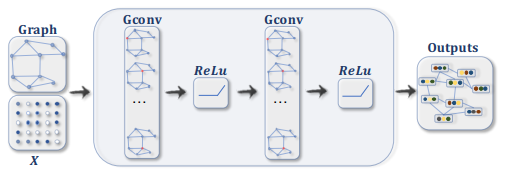
\includegraphics[width=0.95\textwidth]{04-convgnn.png}
    \caption[Examplary GCN architecture for node classification]{\label{img:paper01gcn}{Examplary GCN architecture for node classification \cite{wu_comprehensive_2021}}}
\end{figure} 

GCNs enable the modeling of molecular structures by learning node representations through a certain amount of graph convolutional layers. These layers aggregate information from neighboring atoms, allowing the model to learn relationships within graph data. The main point of the functionality of a GCN is the ability to weight these aggregations, highlighting more important atoms and interactions. \cite{zhang2019graph} Figure \ref{img:paper01gcn} shows an examplary architecture for a GCN: graph data is used as input, the GCN consists of two convolutional layers where ReLu is used as activation function and the output is a predicted property of the input data. \\
The architecture of GCNs involves iterative information propagation through the graph. Each layer computes a weighted sum of neighboring node features, producing node representations. The weight parameters are learned during the training of the model, allowing the GCN to adapt to the characteristics of the respective graph dataset. GCNs are especially effective when working with molecular structures, because the hierarchical structure of a GCN enables the learning of global information, which is required for having a holistic understanding of molecular structures and perform tasks effectively. \cite{wu_comprehensive_2021, zhang2019graph} \\

For the general use of GNNs and other application fields, a total of eight different approaches of GNNs could be identified: the previously explained GCNs, GraphSAGE (Sample and Aggregated), Recurrent Graph Neural Networks (RecGNN), Spatial-temporal Graph Neural Networks (STGNN), Graph Attention Networks (GAN), Graph Isomorphism Networks (GIN), Graph Symmetric Neural Network (GraphSNN),  and Graph Autoencoder (GAE). While AttentiveFP is a specific GAN, the structure and functionality of GANs is similar to that of AttentiveFP described above \cite{xiong_pushing_2019}. For reasons of focus, only the RecGNNs and GAEs are discussed below. \\

Recurrent Graph Neural Networks (RecGNNs) extend the possibilities of traditional GNNs by using both graph-based and recurrent components. Thereby, temporal information and sequential patterns within graphs can be captured. At each time step, the model updates node representations using graph convolutional layers and captures the structure of the evolving graph. Simultaneously, recurrent units capture a memory of past states, which enables the model to save information for a certain time step. The recurrent nature of RecGNNs allows them to learn and represent evolving graph structures. This is especially helpful for a dataset where the relationships between the data show temporal dynamics, e.g. in time-sensitive domains. \cite{li2017diffusion,hajiramezanali2019variational} \\

Designed for learning representations of graph-structured data, Graph Autoencoders are neural network models that are a tool especially helpful for the reconstruction of nodes and graphs. GAEs encode graph-structured input into low-dimensional vectors. By doing so, the essential structural features are captured while the graph typology is preserved. This approach is to be classified as unsupervised learning and supports GAEs in applications like link prediction or anomaly detection. The architecture of GAEs consist of an encoder and a decoder. The encoder maps nodes or graphs to lower-dimensional representations, while the decoder reconstructs the original input from the previously created embeddings. Similar to other variants of GNNs like the RecGNNs, GAEs leverage graph convolutional layers to aggregate information from neighboring nodes during encoding, facilitating the learning of meaningful representations. \cite{li2021adaptive, zhang2021graph}

\subsection{Development of the GNN}
After gaining insight into different architectures and approaches of GNNs in the literature, in the following the development of the GNN for the prediction of potential energy surfaces will be explained. In the course of this paper, a GCN is developed and used with the QM9 Dataset \cite{noauthor_torch_geometricdatasetsqm9_nodate}. In addition, the developed model was trained a second time using a data set containing only water molecules. This will be used to compare the performance of different data sets on the models. The development of the GCN was based on the established CRISP-DM process \cite{wirth2000crisp}, which is explained step by step below. \\

In the initial Phase, the Business Understanding, the goal is to understand the research objectives and requirements. In view of the advancing climate change, the reduction environmental pollution plays an important role for humankind \cite{amin_hydrogen_2022}. This includes the search for scalable and cost-effective renewable energy storage solutions, e.g. like the conversion of electricity to hydrogen as well as the reverse combustion process \cite{kilkis_research_2019}. For this purpose, new materials are being investigated, to enable efficient catalytic processes in the field of hydrogen production \cite{chen_waste-derived_2023}. Machine Learning Methods, like GNNs, are used to simulate and calculate catalytic properties like the prediction of potential energy surfaces \cite{tran_open_2023}. Therefore, the goal of the developed GNN in this paper is to predict the potential energy surfaces of different molecules. \\

The focus of the second step, namely Data Understanding, is to gain insight into the given dataset. The QM9 Dataset consists of approximately 130,000 molecules with 19 regression targets \cite{noauthor_torch_geometricdatasetsqm9_nodate}. 
Within all the different molecules, there are five potential atom types like Carbon and Oxygen and four different types of chemical bonds between them (single bond, double bond, etc.) \cite{menonunderstanding}. For the usage of the GNN, the molecules are transformed, whereas the atoms form the nodes of the graph and the edges are described through the chemical bonds between the atoms. The relevant regression target for the prediction of potential energy surface is the seventh target of the QM9 Dataset, the Internal energy at 0K. The water dataset contains only water molecules with oxygen and hydrogen atoms. In summary, there are approximately 36,000 water molecules in this dataset with different atomic positions or coordinates. Therefore, compared to the QM9 dataset, the water dataset is not as complex in terms of the number of different atoms and chemical bonds and also in the general size of the dataset. The water data set is also used to predict the potential energy surface. \\

In the third step, the available data will be prepared to be able to train the developed GCN. The data preparation includes at first the extraction of all relevant information from the dataset, which is in this case the atoms, the cartesian coordinates, and the Internal energy at 0K. For better results of with the model prediction, the target variables are normalized with the help of their mean and standard deviation. Another important step in the data preparation is the conversion of the coordinates into inverse pairwise distance, so that the GCN understands the spatial relationships like translation and rotation invariance between the atoms in the molecular structure. The same procedure goes for the water dataset.\\

After the data preparation, the GNN architecture is implemented during the modeling phase of the CRISP-DM process. The GNN consists of two convolutional layers, with the before prepared nodes, edges and features as well as the initialized weights as input parameters. The activation function is LeakyRelu. The neural network is implemented with the PyTorch Python package. Before the training, the dataset is randomly split into training and validation dataset, for the evaluation of the model in the next step.\\

The fifth phase describes the evaluation of the developed model, where the performance of the model is assessed with the validation dataset. With the help of the Adam optimizer algorithm, also implemented in PyTorch, the model is optimized during training. With this procedure, the ability of the model to generalize and make accurate prediction on data other than the training data is enhanced. Since the prediction of the potential energy surfaces is a regression task, the performance of the model can be measured by using different regression performance metrics. The following performance metrics are used: Model Training Time (lower is better), Mean Squared Error (lower is better), Root Mean Squared Error (lower is better) and the $R^2$-Score (higher is better). In the following, the performance metrics are evaluated by comparing the performance of a baseline (non-graph-based) neural network architecture with the implemented GCN architecture, where the different approaches are trained individually for each dataset. Table \ref{tab:paper01performancecomparisonqm9} lists the computed metrics for the training with the QM9 dataset.

\begin{table}[h!]
    \centering
    \captionsetup{justification=centering}
    \resizebox{\textwidth}{!}{
        \setlength{\tabcolsep}{1.5em}
        {\renewcommand{\arraystretch}{1.5}% for the vertical padding
            \begin{tabular}{p{7cm} l l}
                \hline
                 \textbf{Parameter} & \textbf{Baseline Model} & \textbf{Graph-based Model} \\
                 \hline
                   Training time &  6 min 17.1s & 9 min 2.4s  \\
                   Mean Squared Error (MSE) & 365484.59 & 11513.64 \\
                   Root Mean Squared Error (RMSE) & 604.553 & 107.30 \\
                   $R^2$-Score ($R^2$) & 0.6904  & 0.9902 \\
                   \hline
               \end{tabular}
           }
       }
       \caption[Comparison of performance metrics of the developed model (QM-9 dataset)]{\label{tab:paper01performancecomparisonqm9} Comparison of performance metrics of the developed model [QM-9 dataset]}
\end{table}

As shown in the Table, training the baseline model with similar hyperparameters to the GCN takes about 3 minutes less than training the GCN. However, the measurement of MSE and RMSE shows that the results of the GCN are much more accurate than the results of the baseline model, e.g. the RMSE of the GCN is about 6 times smaller than the RMSE of the baseline architecture. Comparing the overall accuracy using the $R^2$ score shows that the baseline model has an accuracy of 69\% while the GCN has an accuracy of 99\%, indicating a very accurate fit between the predictions and the actual data. The difference in accuracy between the two models can be seen by comparing the Figures \ref{fig:sfig1} and \ref{fig:sfig2}.\\

The following Table \ref{tab:paper01performancecomparisonwater} compares the performance metrics of the baseline and GCN models trained on the water dataset. It can be seen that there is not much difference in the training time of the different models, while interestingly the GCN trains faster than the baseline model with the same hyperparameters. However, the baseline neural network provides more accurate results, with the MSE and RMSE values being smaller than those of the GCN. Also, the accuracy of the baseline model is 99.1\%, while the accuracy of the GCN is only 97.6\%.

\begin{table}[h]
    \centering
    \captionsetup{justification=centering}
    \resizebox{\textwidth}{!}{
        \setlength{\tabcolsep}{1.5em}
        {\renewcommand{\arraystretch}{1.5}% for the vertical padding
            \begin{tabular}{p{7cm} l l}
                \hline
                 \textbf{Parameter} & \textbf{Baseline Model} & \textbf{Graph-based Model} \\
                 \hline
                   Training time &  1 min 38.3s & 1 min 26.9s \\
                   Mean Squared Error (MSE) & 0.0000612 & 0.0014 \\
                   Root Mean Squared Error (RMSE) & 0.0078 & 0.0373 \\
                   $R^2$-Score ($R^2$) & 0.9991  & 0.9756 \\
                   \hline
               \end{tabular}
           }
       }
       \caption[Comparison of performance metrics of the developed model (water dataset)]{\label{tab:paper01performancecomparisonwater} Comparison of performance metrics of the developed model [water dataset]}
\end{table}

While the training of the models with the QM9 dataset shows very different results, the Figures of \ref{fig:sfig3} and \ref{fig:sfig4} show that there is only a small difference in terms of accuracy when training a baseline and a GCN model with the simpler water dataset.


\begin{figure}[h!]
    \begin{subfigure}{.5\textwidth}
     \captionsetup{justification=centering}
      \centering
      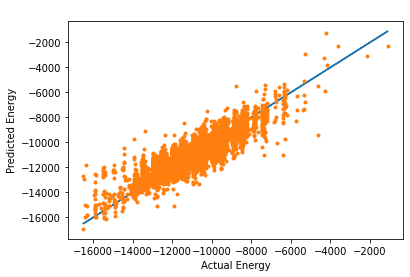
\includegraphics[width=.8\linewidth]{qm9-nn-result.png}
      \caption{QM9 dataset classical neural network approach}
      \label{fig:sfig1}
    \end{subfigure}%
    \begin{subfigure}{.5\textwidth}
      \centering
      \captionsetup{justification=centering}
      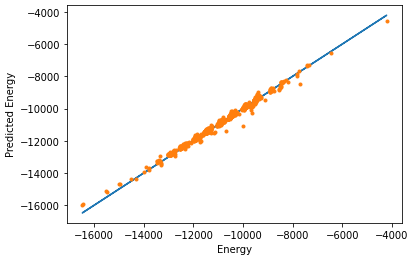
\includegraphics[width=.8\linewidth]{qm9-gnn.png}
      \caption{QM9 dataset graph-based neural network approach}
      \label{fig:sfig2}
    \end{subfigure}
    \begin{subfigure}{.5\textwidth}
        \centering
        \captionsetup{justification=centering}
        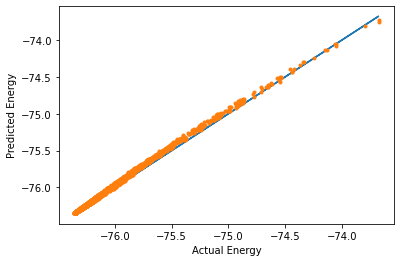
\includegraphics[width=.8\linewidth]{water-nn.png}
        \caption{Water dataset classical neural network approach}
        \label{fig:sfig3}
      \end{subfigure}
      \begin{subfigure}{.5\textwidth}
        \captionsetup{justification=centering}
        \centering
        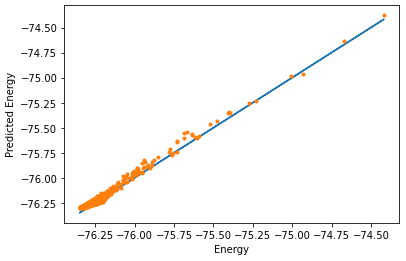
\includegraphics[width=.8\linewidth]{water-gnn.png}
        \caption{Water dataset graph-based neural network approach}
        \label{fig:sfig4}
      \end{subfigure}
    \caption{Comparison of actual and predicted energy from the different datasets}
    \label{fig:plotsofresults}
    \end{figure}

To summarize the evaluation, it can be said that the use of a GCN architecture is particularly useful when the dataset is complex and contains different atoms and chemical compounds, as is the case with the QM9 dataset. In contrast, the use of a basic neural network architecture is recommended for rather simple datasets, such as the water dataset used previously. \\

During the last phase of the CRISP-DM process, the developed and evaluated GCN can be deployed and make use of the knowledge gained. In the course of this paper, the developed GCN is a prototype and will be further used for the comparison to other machine learning models in the context of potential energy surface prediction. 

\section{Conclusion}
Overall, the conducted research process has proven to be suitable for the literature review, followed by the development of the GCN for molecular property prediction. In this chapter, the results are summarized and critically reflected upon, and future research potential is identified. 

\subsection{Summary}

Within the scope of the literature review, in total 11 different architectures or approaches for the implementation of GNNs could be identified and further categorized. Furthermore, an overview over the differences between the identified approaches and architectures was given. Utilizing the information gained in the scope of the literature review, the convolutional approach of a GNN was used for the development of a GNN that predicts the potential energy surface of a molecule. By using the in the discipline of computational chemistry frequently used QM9 dataset for the development of the model, the results can be adapted to other datasets that contain different information, e.g. in form of other molecules. 

\subsection{Critical Reflection}
As mentioned before, the research methodology was suitable for analyzing the findable literature and for the prototypical implementation of the GNN. However, this work also has its limitations. Further approaches or architectures of GNNs could have been investigated to be used for the prediction of potential energy surfaces. By doing so, a comparison between the results, e.g. with measured performance metrics, could have taken place. In addition, the developed GNN could have been tested with other datasets than the QM9 dataset, to be able to evaluate its general validity. These aspects might have identified important requirements that are not included in the current iteration of the prototypical GNN.

\subsection{Outlook}

The insights in gained in this paper provide a starting point for future research. The QM9 dataset, that was used in this paper, provides quantum chemical properties at DFT level. Besides, the prediction of potential energy surfaces and other relevant properties proceeds at the molecular and atomic level. The advancing development of quantum computers raises the question, if machine learning models like GNNs that compute quantum properties like potential surface areas can be realized on quantum computers. While there already exist first approaches of quantum graph neural networks in the literature \cite{verdon_quantum_2019,beer_quantum_2021,ai_decompositional_2023}, the results of the literature review and the developed GNN in this paper serve as a starting point for a further investigation in the field of quantum graph neural networks. 
